% Chapter Template

\chapter{Comments-Observations} % Main chapter title

\label{Chapter7}

Concluding internship's report, I would like to leave some comments regarding:

\begin{itemize}
	\item working environment and my team: Both 
	\item Ability to build a three-layer web application
	\item Good knowledge of Unix based Systems
	\item Basic understanding of both Sql and N0-Sql databases
	\item Ability of problem solving and understanding algorithms complexity
	\item Familiar with GitHub Usage
	\item Ability to work in a team, communicate ideas, be an active member and deliver on time
\end{itemize}


\chapter{Appendix}

\section{Stas NPM package - ReadME.md file}
	\textbf{Install}
	
	\begin{lstlisting}[language=bash]
	$ npm install @freenow-gr/stats$
	\end{lstlisting}
	
	or
	
	\begin{lstlisting}[language=]
	$ yarn add @freenow-gr/stats$
	\end{lstlisting}

	\textbf{Usage}
	
	\begin{lstlisting}[language=JavaScript]
	import {groupStatistics, KPI, resolutions} 
			from "@freenow-gr/stats";
	
	const validMockedData = {
		y2019: {
			m3: {
				d12: {
					h15: {
						CancelledCounter: 1,
						CompletedCounter: 3,
						revenueSum: 258.47,
					},
				},
			},
		},
	};	
	const args = {
		statsObject:validMockedData, 
		startTimestamp: new Date('2018-02-10T15:45:00'), 
		endTimestamp: new Date('2018-02-12T15:45:00'), 
		kpi:KPI.GMV, 
		resolution:resolutions.HOUR
	}
	\end{lstlisting}
	
	\newpage
	In order to run you need to have an object like this:
	
	\begin{lstlisting}[language=JavaScript]
	let result = groupStatistics(args);
	console.log(result);
	//y2018: {
	//	m2: {
	//		d12: {
	//			h15: {
	//				revenueSum: 258.47,
	//				},
	//			},
	//		},
	//	}
	
	\end{lstlisting}
	
	
\section{Landing Page - Responsive in all devices}

The landing page created for mpaineis-vgaineis competition was used from a large amount of Beat and non-Beat users. The page had to be responsive and differently displayed in the variety of mobiles, tablets and desktops, and also to match with the designs given through Zeplin and shown in figure 8.1.

\begin{figure}[H]
	\begin{center}
		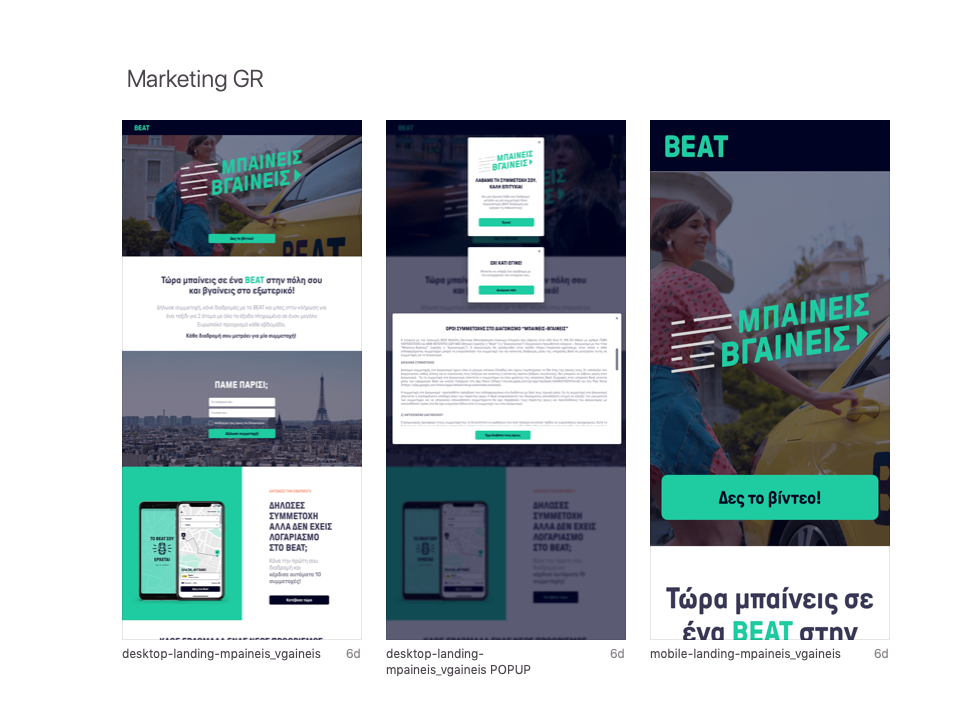
\includegraphics[scale=0.4]{images/my_projects/landing_page/zeplin.png}
	\end{center}
	\caption{Designs of Landing page in Zeplin}
\end{figure}

Following, it is displayed every screen on mobile taken from \url{mpaineis-vgaineis.gr} and in figures 4.4 and 4.5 of Chapter \ref{Chapter5} you can find the same screens in desktop.
\begin{figure}[H]
	\centering
	\subfloat[Header \& Video Display]{{
\includegraphics[scale=0.18]{images/my_projects/landing_page/header-mobile.jpg} }}%
	\qquad
	\subfloat[Description]{{
\includegraphics[scale=0.18]{images/my_projects/landing_page/description-mobile.png} }}%
	\qquad
	\subfloat[Form]{{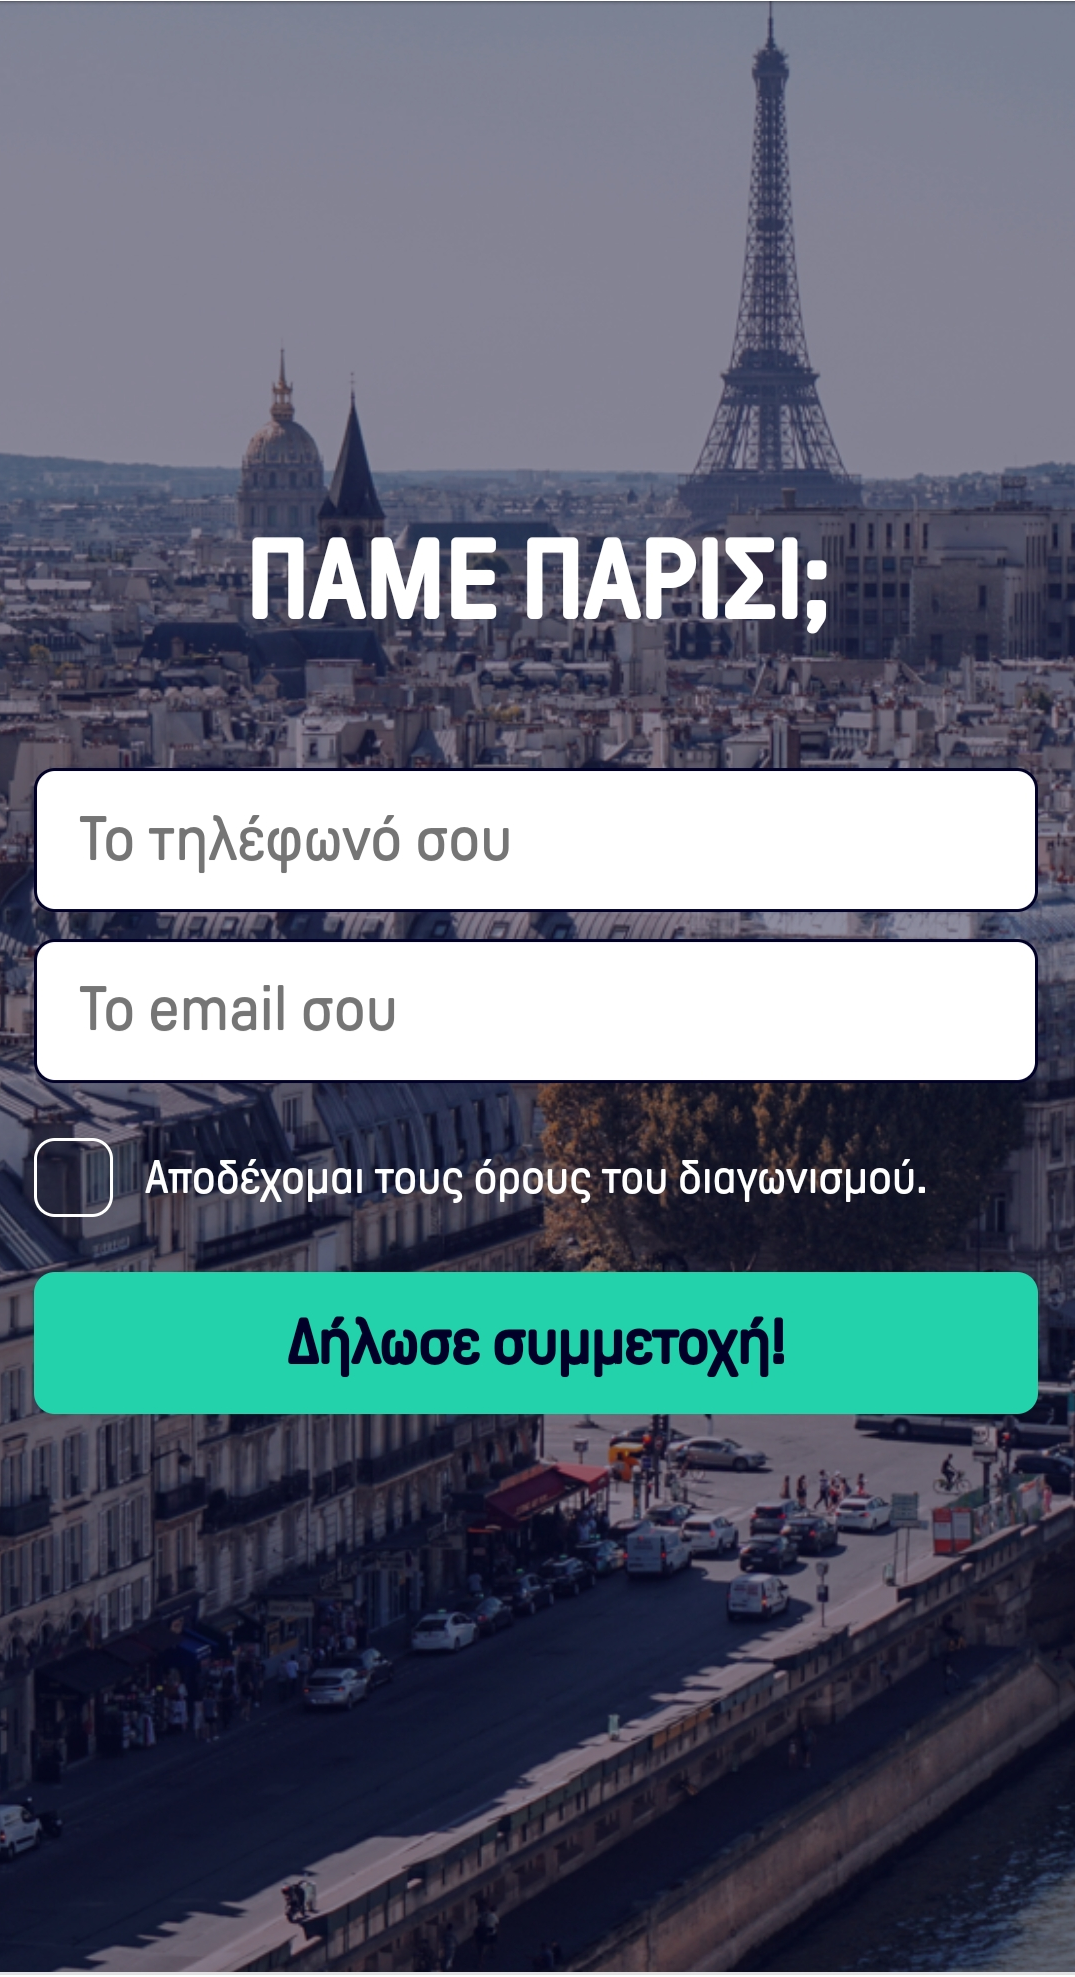
\includegraphics[scale=0.18]{images/my_projects/landing_page/form-mobile.png} }}%
	\caption{
		Landing Page for Competition mpaineis-vgaineis
		\\
		\textbf{Online: } \url{https://mpaineis-vgaineis.gr/}
	}
	\label{fig:example}
\end{figure}

\begin{figure}[H]
	\centering
	\subfloat[App Display]{{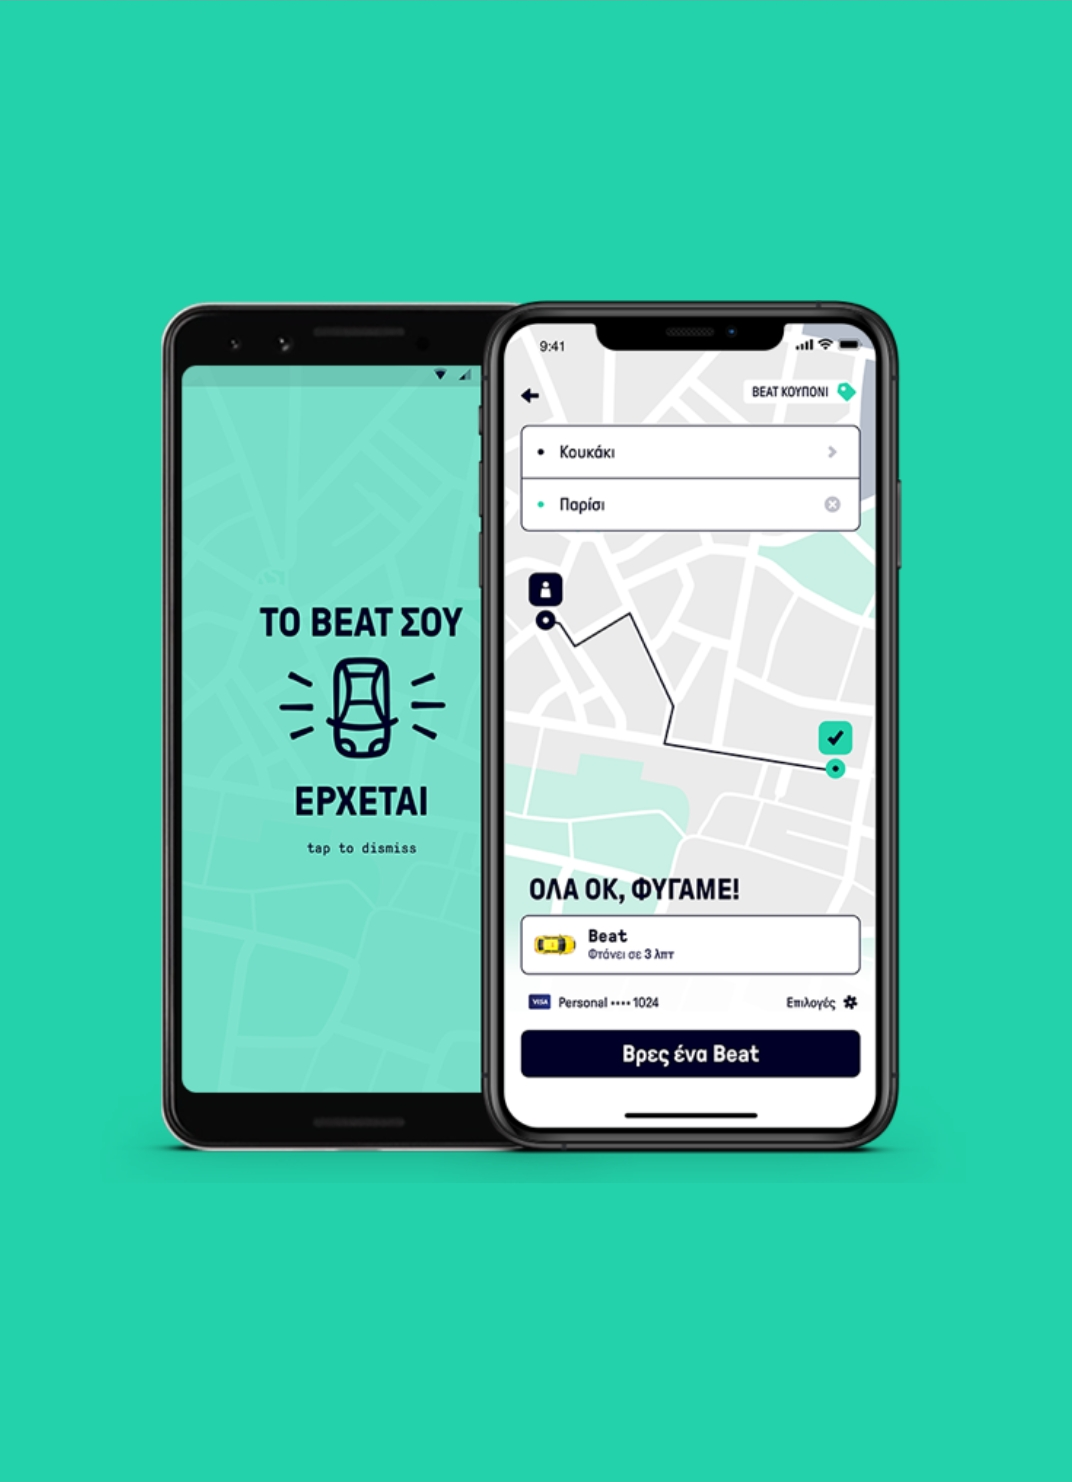
\includegraphics[scale=0.18]{images/my_projects/landing_page/app-mobile.png} }}%
	\qquad
	\subfloat[Download App]{{
\includegraphics[scale=0.18]{images/my_projects/landing_page/app-download-mobile.png} }}%
	\qquad
	\subfloat[Social Media \& Footer]{{
\includegraphics[scale=0.18]{images/my_projects/landing_page/footer-mobile.png} }}%
	\caption{
		Landing Page for Competition mpaineis-vgaineis
		\\
		\textbf{Online: } \url{https://mpaineis-vgaineis.gr/}
	}
	\label{fig:example}
\end{figure}

\begin{figure}[H]
	\centering
	\subfloat[PopUp Confirmation ]{{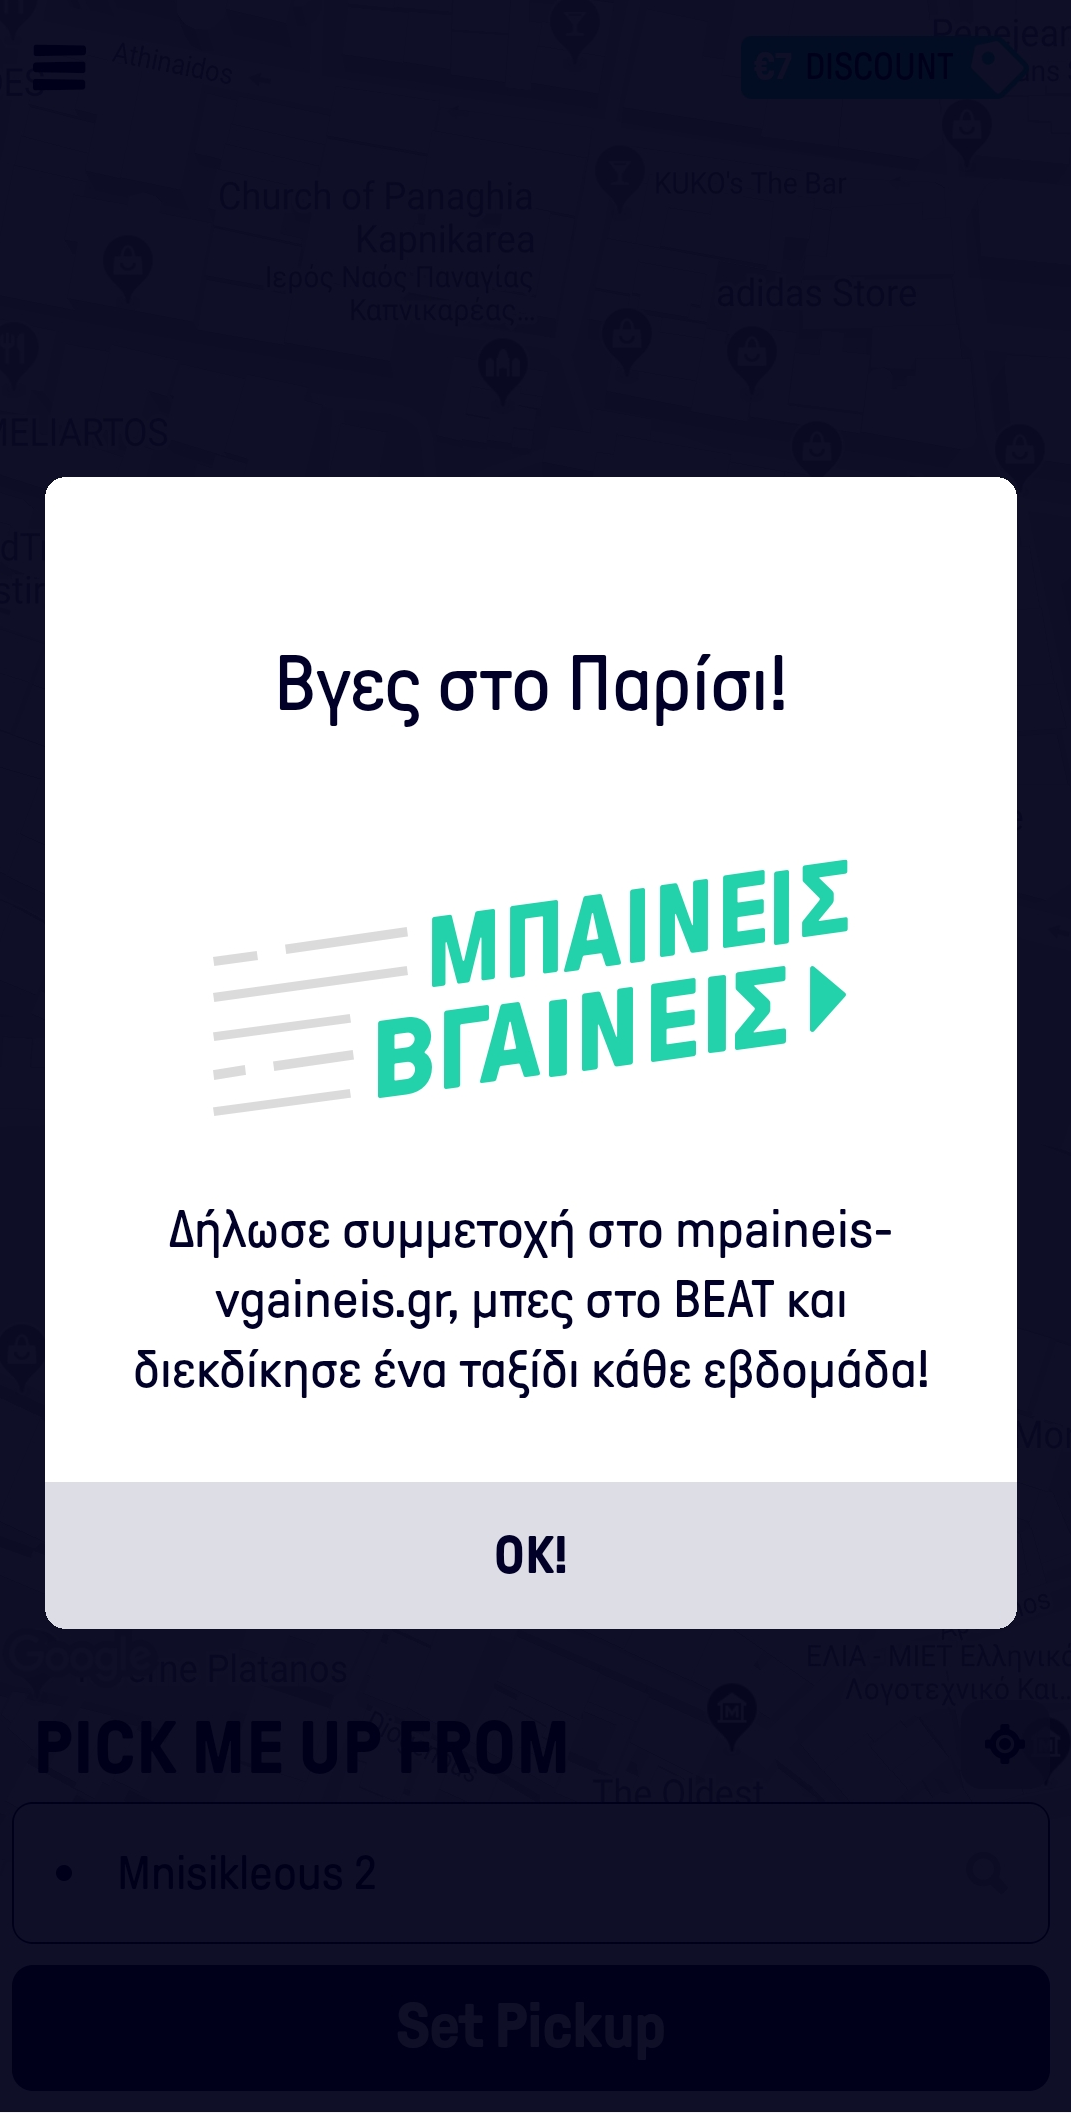
\includegraphics[scale=0.2]{images/my_projects/landing_page/popup-confirmation-mobile.png} }}%
	\qquad
	\subfloat[PopUp Limits]{{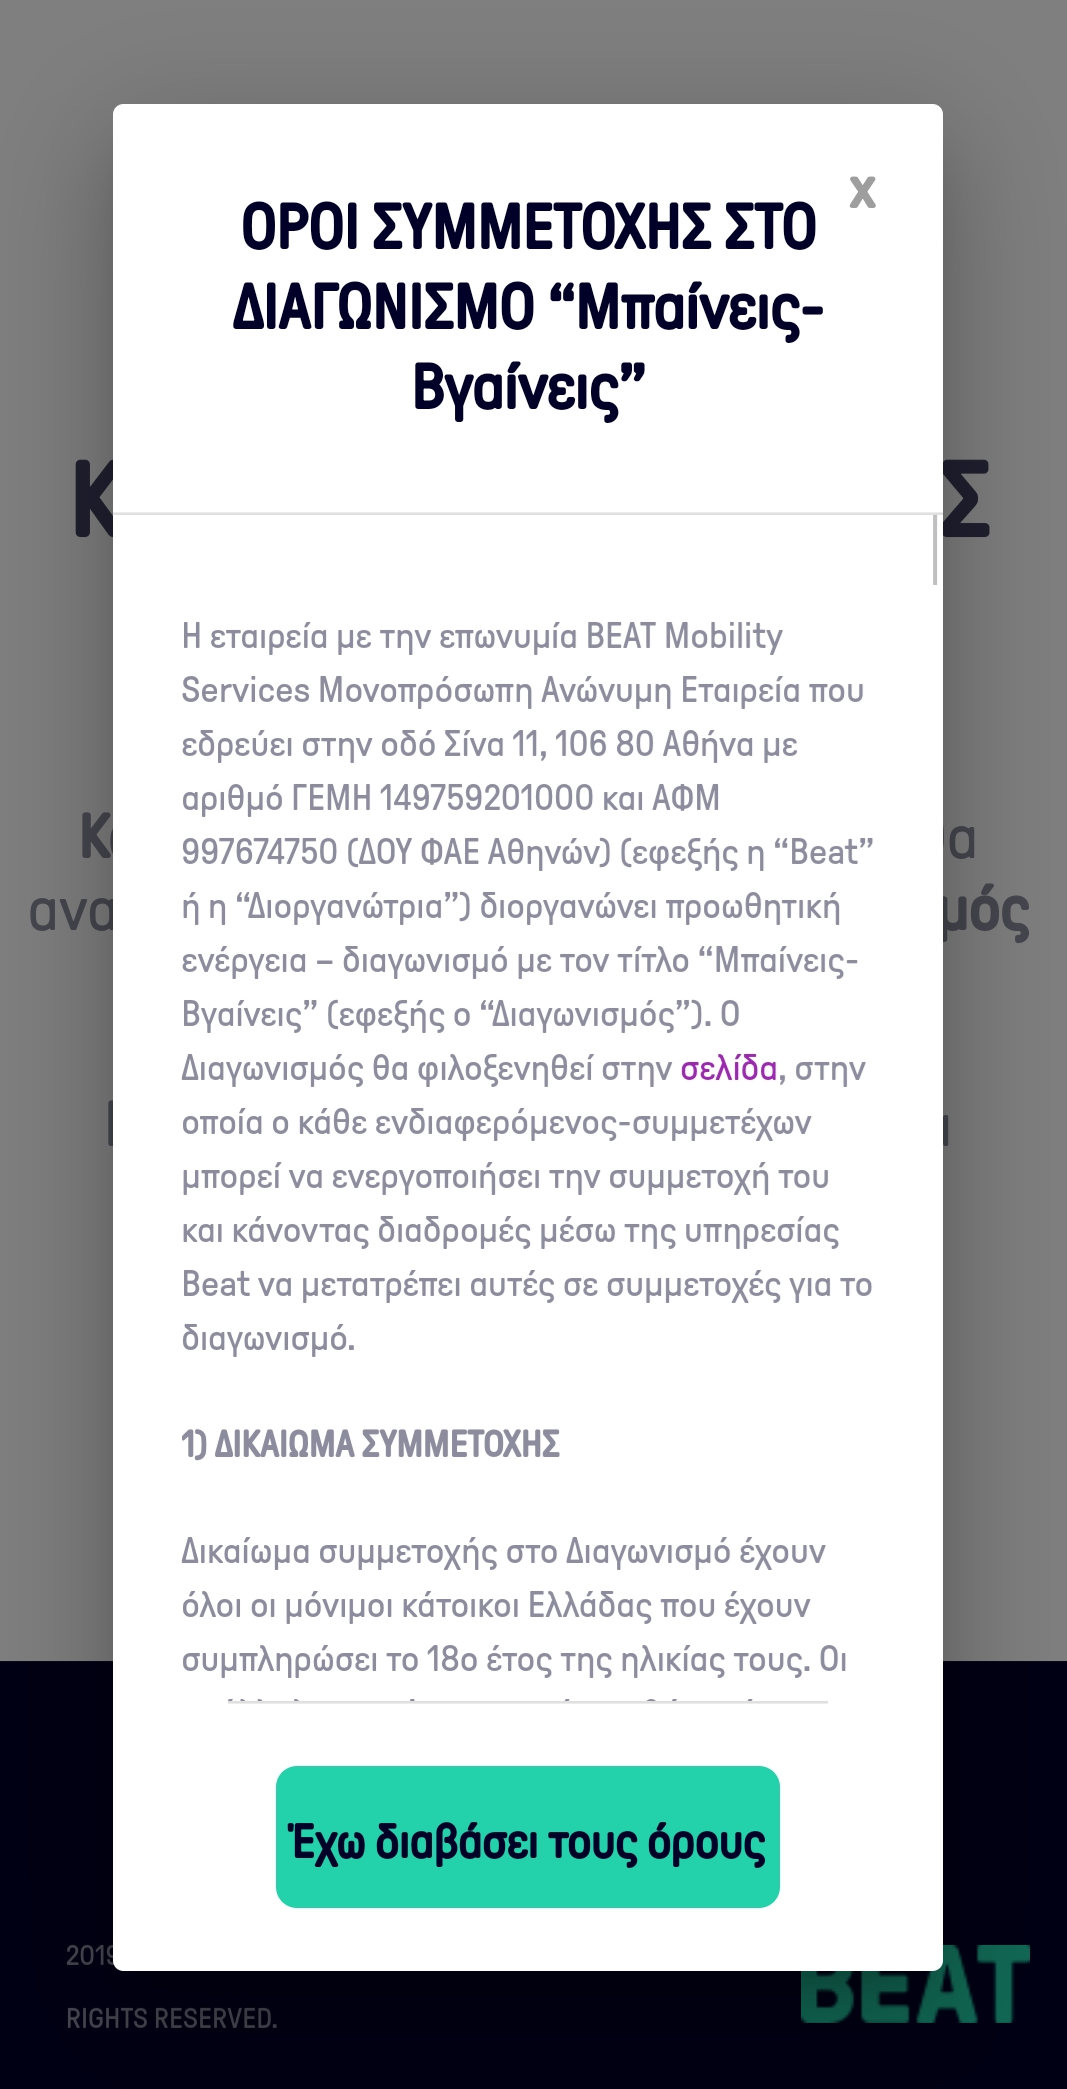
\includegraphics[scale=0.2]{images/my_projects/landing_page/limits-mobile.png} }}%
	\caption{
		Landing Page for Competition mpaineis-vgaineis
		\\
		\textbf{Online: } \url{https://mpaineis-vgaineis.gr/}
	}
	\label{fig:example}
\end{figure}
